%%This is a very basic article template.
%%There is just one section and two subsections.
\documentclass{article}
\usepackage{graphics}
\usepackage{graphicx}
\usepackage{url}
\usepackage[utf8]{inputenc}
\usepackage[spanish]{babel}
\usepackage{myCoverPage}
\usepackage{fancyhdr}
\usepackage{color}
\usepackage{colortbl}
\usepackage{colourlist}


\usepackage{tocloft}

%If invoked with [final] then fixes and notes will be not shown
\usepackage[final,inline]{fixme}
\usepackage{hyperref}

% configuración del paquete hyperref
\hypersetup{    pdfauthor = {/Elena Mor'on Muela},
		pdftitle = {},
		colorlinks={true},
		pdfstartview={FitV},
		linkcolor={blue4},
		citecolor={blue4},
		urlcolor={blue4}
}




\usepackage[a4paper]{geometry}
\oddsidemargin -0.04cm   % read Lamport p.163
\evensidemargin -0.04cm  % same as oddsidemargin but for left-hand pages

\renewcommand{\CoverPageHeader}{%
    \parbox{\linewidth}{%
        \tiny
   
    }%
}

% Control de lneas viudas y huérfanas
\clubpenalty=100000
\widowpenalty=10000
\displaywidowpenalty=1000
\looseness=1

%-----------------------------------------------------------------------------%
%
% Formato de las cabeceras
%
\pagestyle{fancyplain}

\lhead[
        \fancyplain{}
	    {\textrm{\textbf{\thepage}\hspace{4mm}\small\leftmark}}]
        {\fancyplain{}
        {\textrm{\footnotesize\textcopyright\ GSO}}}
\rhead[
        \fancyplain{}
        {\textrm{\footnotesize\textcopyright\ GSO}}]
        {\fancyplain{}
        {\textrm{\small\rightmark\hspace{4mm}\normalsize\textbf{\thepage}}}}
\cfoot[]{} % En el pie de página no ponemos nada
\renewcommand{\headrulewidth}{0.1mm}

\graphicspath{\resources}
%¿No debería ser Anteproyecto de Trabajo de Fin de Carrera?
\renewcommand{\CPTitle}{\LARGE Anteproyecto de Fin de Grado.\\\huge\sc Ley de Prevención del blanqueo de capitales}
\renewcommand{\CPAuthor}{Autor: \ Elena Morón Muela\\Tutor: \'Oscar Garc\'ia
Población}
\renewcommand{\CPDireccion}{Universidad de Alcalá\\Escuela
Politécnica Superior\\Departamento de Automática\\}
%\newcommand{\tituloTFC}{Sistema integrado de información geográfica para la gestión de expropiaciones}
%¿para que sirve la siguiente línea?
%sale un source undefined debajo del email.
\newcommand{\ssh}{\texttt{ssh}}


\begin{document}
\title{Propuesta de Proyecto fin de Carrera}
\pagenumbering{arabic}
\setcounter{page}{2}
\cleardoublepage

\setcounter{tocdepth}{2}
\tableofcontents
\listoffixmes



\section{Introducción}
Este documento se corresponde con el anteproyecto de fin de grado para la titulación de Ingeniería Informática. El título elegido es Ley de prevencción del blanqueo de capitales.
En principio se va explicar que objetivos tiene este proyecto, tanto en el desarrollo como en el aprendizaje de nuevas tecnologías. Se incluye también una descripción con estos mismos bloques.
Se presentará un diagrama de Gantt que mostrará el plan de trabajo a seguir, además del plan de trabajo se hablará de metodología que se usará para el desarrollo del proyecto.
Por último una bibliografía para indicar que fuentes han sido utilizadas.  


 


\section{Objetivos y campo de aplicación.}
Explicaré que objetivos han movido el desarrollo de este proyecto, como se comentaba en la introducción se van a dividir en dos bloques. El propio desarrollo de la aplicación y los conocimientos que se quieren adquirir.
En el ámbito de la aplicación son realizar una aplicación informática multiplataforma que permita coordinar las labores de auditoría de una empresa de auditoría de cuentas.
Por la parte de aprendizaje explorar nuevas tecnologías WEB de desarrollo, tanto para la interacción con el usuario como para el almacenamiento y procesamiento de los datos en el lado del servidor.



\section{Descripción del trabajo}
En la descripción se va hablar de los bloques que tiene la propia aplicación en el lado del desarrollo. Se dispone de dos grandes bloques conocidos como backend y frontend, podemos la descripción de estos con la siguiente imagen.
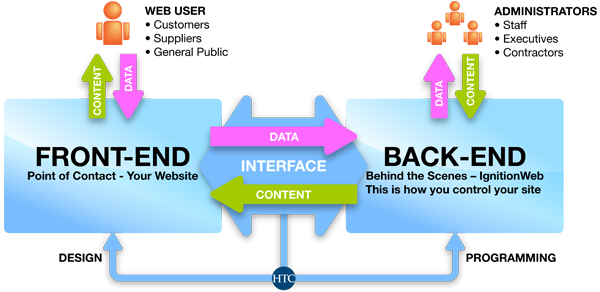
\includegraphics{front_back}






\section{Metodología y plan de trabajo}



\section{Medios}




\nocite{*}
\bibliographystyle{plain}
\addcontentsline{toc}{section}{Referencias}


\end{document}
